\documentclass[conference,a4paper,10pt]{IEEEtran}
\IEEEoverridecommandlockouts

\usepackage{cite}
\usepackage{amsmath,amssymb,amsfonts}
\usepackage{graphicx}
\usepackage{textcomp}
\usepackage{xcolor}
\usepackage{booktabs}
\usepackage{tabularx}
\usepackage{array}
\usepackage{tikz}
\usepackage[hyphens]{url}
\usepackage{placeins}
\usepackage{fancyhdr}
\usepackage[hidelinks,bookmarks=false]{hyperref}
\usetikzlibrary{arrows.meta,calc,fit,positioning,decorations.pathreplacing}
\urlstyle{same}
\makeatletter
\def\UrlBigBreaks{\do@url@hyp}
\g@addto@macro{\UrlNoBreaks}{\do\:}
\makeatother

% ICCIT camera-ready notices appear only on the title page.
\fancypagestyle{iccitfirstpage}{%
  \fancyhf{}%
  \fancyhead[L]{\footnotesize\raisebox{0pt}[0pt][0pt]{\shortstack[l]{%
    2026 29th International Conference on Computer and Information Technology (ICCIT)\\
    18-20 December 2026, Cox's Bazar, Bangladesh}}}%
  \fancyfoot[L]{\footnotesize
    979-8-3195-0171-4/26/\$31.00~\copyright{}2026 IEEE}%
  \renewcommand{\headrulewidth}{0pt}%
  \renewcommand{\footrulewidth}{0pt}%
}
\pagestyle{empty}

\definecolor{jbblue}{RGB}{35,91,133}
\definecolor{jbteal}{RGB}{35,116,105}
\definecolor{jbamber}{RGB}{171,106,29}
\definecolor{jbred}{RGB}{158,48,48}
\definecolor{jbgray}{RGB}{241,243,245}
\definecolor{jbink}{RGB}{39,50,56}

\def\BibTeX{{\rm B\kern-.05em{\sc i\kern-.025em b}\kern-.08em
    T\kern-.1667em\lower.7ex\hbox{E}\kern-.125emX}}

\begin{document}

\title{Islands of Reach: A Censorship-Resistant Federated Forum for
National Internet Blackouts}

\author{%
  \IEEEauthorblockN{Tasmir Hossain Zihad\quad Sarwad Hasan Siddiqui\quad Rezuan Mustafa Hasan}
  \IEEEauthorblockA{Khulna University of Engineering \& Technology\\
    Khulna 9203, Bangladesh\\
    \texttt{tasmir@tuta.io}\quad \texttt{sarwad015@gmail.com}\quad
    \texttt{hasanideal2002@gmail.com}}
}

\maketitle
\thispagestyle{iccitfirstpage}

\begin{abstract}
A partial Internet shutdown may lead to the cutoff of international traffic but still leave some domestic IP routes available. We built Jagoo Bahee to test whether forum servers can accept signed posts locally and share them over those routes. Servers verify incoming messages, issue signed receipts, and fetch missing records from peers. A relay connected to both networks checks messages before forwarding them. In a single-host Docker testbed, all 20 certificate--community--post sequences arrived over the direct route, and all 20 new sequences arrived through the relay after the cut. Median post delivery time rose from 0.735 to 1.732 seconds. All ten posts arrived in the unshaped control and in each of the five impairment conditions. On a bandwidth-limited link with packet loss, Jagoo Bahee and a minimal ActivityPub inbox each delivered all 20 posts. With inbound federation ports blocked, Jagoo Bahee pulled all ten posts over outbound connections. The push-only baseline delivered none within its retry budget. The TypeScript, Rust, and Python decoders agreed on all 20,000 fuzz-test cases, including generated and mutated inputs. These results show that forum servers can resume sharing posts over surviving routes in a controlled testbed. Performance during a real shutdown or a sustained denial-of-service attack remains untested.
\end{abstract}

\begin{IEEEkeywords}
Federated systems, Internet shutdowns, network partitions, signed objects, store-and-forward.
\end{IEEEkeywords}

\section{Introduction}

Deliberate Internet shutdowns may restrict bandwidth, destinations, or protocols while leaving domestic IP routes available \cite{ooni2025bangladesh,bischof2023shutdowns}. Baltra et al.~\cite{baltra2024connectivity} distinguish \emph{connectivity islands}, which retain local connectivity while cut off from the Internet core, from \emph{peninsulas}, which retain partial reachability to the core. We ask whether independent forum servers can accept signed posts locally and reconcile their logs over the remaining IP paths.

Circumvention proxies \cite{bocovich2024snowflake} and device-to-device meshes \cite{kamali2025anix,lerner2016rangzen,pradeep2022moby} address different connectivity conditions. We study secure federation under partial Internet connectivity with Jagoo Bahee, a federated forum prototype. We make four contributions.
\begin{enumerate}
  \item A byte-preserving admission path that applies the same core validation checks to local and federated envelopes.
  \item Caller-driven delivery, streaming, and backfill via outbound connections with asymmetric connectivity.
  \item A quota-controlled, dual-homed relay that verifies signed envelopes before forwarding them.
  \item An evaluation of route cuts, network impairments, hop scaling, admission under load, delivery against a minimal ActivityPub inbox, and cross-language wire-format agreement.
\end{enumerate}
The design requires surviving IP paths. Operators can still refuse admission and observe relay traffic.

\section{Background and Research Gap}
\label{sec:background}

ActivityPub sends activities to actor inboxes \cite{activitypub}, AT Protocol uses signed repository commits \cite{atproto}, and Nostr uses signed events and relays \cite{nostr}. Snowflake needs a reachable rendezvous point \cite{bocovich2024snowflake}. Anix, Rangzen, and Moby use device-to-device communication when IP connectivity is limited or unavailable \cite{kamali2025anix,lerner2016rangzen,pradeep2022moby}. In the setting we study, independently operated servers retain domestic IP paths linking islands or peninsulas. Our design uses canonical wire validation, outbound synchronization, and quota-limited relaying. During admission, a server also checks the timestamp against its clock, looks for prerequisite records, and applies the relevant anti-abuse policy.

Certificate Transparency offers Merkle inclusion and consistency proofs \cite{rfc6962,rfc9162}. PeerReview uses verifiable logs for accountability \cite{haeberlen2007peerreview}, and CoSi uses witness co-signing \cite{syta2016cosi}. Our threat model covers malformed inputs, replay attacks, and servers that later conceal objects they admitted. A signed receipt attests that a server accepted the identified content.

\section{System Design}
\label{sec:design}

\subsection{Architecture and scheduling}

\begin{figure*}[!t]
  \centering
  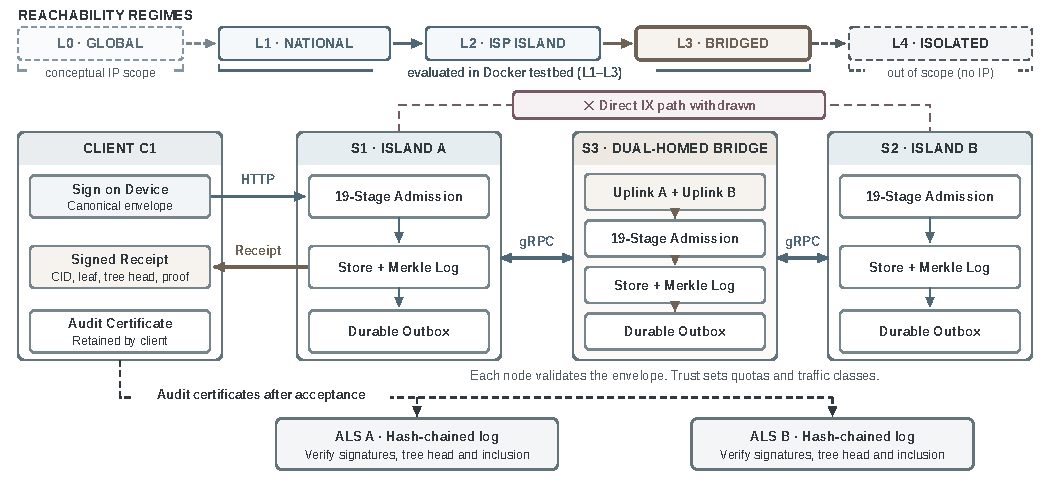
\includegraphics[width=.80\textwidth]{figures-v2/fig1-system-architecture-camera.pdf}
  \caption{Clients, validating island nodes, dual-homed relays, and external audit-log services (ALSs). The upper bar marks the conceptual global regime (\texttt{L0}), the Docker test scenarios (\texttt{L1--L3}), and total isolation (\texttt{L4}, outside the evaluation). Clients send audit certificates outside the admission path.}
  \label{fig:architecture}
\end{figure*}

Clients submit envelopes over HTTP, and servers federate using gRPC (Fig.~\ref{fig:architecture}). The dual-homed bridge uses one address per island. The trust configuration sets peer quotas and traffic classes. The bridge applies the full admission pipeline, stores the relayed objects, and signs its own receipts. It applies quotas by \texttt{(source uplink, destination uplink, priority)} and skips the supplying peer during fan-out. Each node drains its durable outbox in \texttt{(priority, sequence)} order and uses separate delivery leases for each combination of peer and message plane so a stalled connection does not block other peers. Clients send audit certificates to an audit-log service (ALS) outside the write path.

\subsection{Signed objects and admission}

An envelope carries its version, plane, domain tag, author key and algorithm, optional parent, scope, creation timestamp, 16-byte nonce, priority, payload, and anti-abuse fields. Receivers accept timestamps from seven days before their local clock to ten minutes ahead. Ed25519 signatures \cite{bernstein2012ed25519} and SHA-256 content identifiers bind the canonical encoding of fields 1--12. Jagoo Bahee uses a restricted protobuf profile \cite{protobufnotcanonical} that requires ascending field order, minimal varints, default omission, Unicode Normalization Form C (NFC) for strings, and rejection of unknown fields. Receivers reject any mismatch between received and re-encoded envelope bytes before decoding the payload. The byte comparison rejects noncanonical encodings of otherwise valid signed content.

\begin{figure}[!t]
  \centering
  {\footnotesize
  \begin{tabularx}{\columnwidth}{@{}lX@{}}
    \toprule
    \textbf{Stage} & \textbf{Check or action} \\
    \midrule
    Before stage 1 & HTTP rate limit or \textsc{Deliver} parse and quota check \\
    \midrule
    1--2 & Size, parse, canonical re-encoding \\
    3--7 & Version, domain, plane, size, algorithm, priority \\
    8--10 & Clock window, signature, certificate \\
    11--12 & Content-ID deduplication and nonce replay check \\
    \midrule
    13 & Origin anti-abuse policy \\
    14--15 & Authorization and semantic validation \\
    16--18 & Atomic storage, projection, Merkle append, and signed receipt \\
    19 & Durable fan-out to eligible peers \\
    \bottomrule
  \end{tabularx}}
  \caption{Admission pipeline for local and federated envelopes.}
  \label{fig:pipeline}
\end{figure}

HTTP rate limiting takes place before admission (Fig.~\ref{fig:pipeline}). The gRPC \textsc{Deliver} handler parses each frame and checks the peer quota before running the admission checks. Responses fetched by a caller go directly to the admission checks. Stages~1--12 are read-only and check canonical encoding, domain and plane rules, the timestamp window, signatures, certificates, duplicate content identifiers, and nonce replay. Stage~13 applies the originating node's anti-abuse policy. Federated arrivals skip this stage because anti-abuse tokens are tied to the origin's secrets. Stage~14 authorizes the operation against projections (local state derived from accepted records), and Stage~15 checks domain semantics. Stages~16--18 atomically store the raw envelope, update projections, add a Merkle leaf, and sign the receipt. Idempotent retries return the stored receipt. The server treats nonce reuse for a non-idempotent operation as replay. A database uniqueness constraint prevents duplicate entries when push delivery and backfill race.

\subsection{Partition-aware federation}

Three caller-initiated gRPC methods govern replication: \textsc{Deliver} pushes batches of accepted envelopes, \textsc{StreamActivities} reads a finite snapshot from a durable cursor, and \textsc{Backfill} fetches missed entries from a resumable log position. Since the caller initiates each RPC, even a node that is behind carrier-grade NAT or a firewall that blocks inbound connections can communicate in both directions through outbound connections. To begin outbound synchronization, the operator must know at least one reachable peer address. A catch-up timer polls every 2\,s by default; outbound-only nodes poll known peers continuously, whereas listening nodes trigger catch-up when inbound activity is stale for two polling intervals (4\,s). In the route-cut topology (Fig.~\ref{fig:topology}), the dual-homed bridge carries cross-island traffic once the shared exchange disappears.

\begin{figure}[!t]
  \centering
  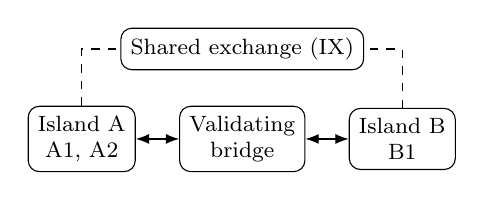
\begin{tikzpicture}[font=\footnotesize, >=Latex, node distance=5.5mm,
      box/.style={draw, rounded corners, align=center, inner sep=3.5pt}]
    \node[box] (bridge) {Validating\\bridge};
    \node[box, left=of bridge] (a) {Island A\\A1, A2};
    \node[box, right=of bridge] (b) {Island B\\B1};
    \node[box, above=4.5mm of bridge] (ix) {Shared exchange (IX)};
    \draw[<->] (a) -- (bridge);
    \draw[<->] (bridge) -- (b);
    \draw[dashed] (a.north) |- (ix.west);
    \draw[dashed] (b.north) |- (ix.east);
  \end{tikzpicture}
  \caption{Four-node route-cut testbed. Withdrawing the dashed exchange path leaves A1 and B1 connected via the dual-homed bridge while A2 remains on island~A.}
  \label{fig:topology}
\end{figure}

Default RPC deadlines are 5\,s for control calls, 15\,s for delivery, and 30\,s for backfill. Delivery propagates cancellation through \texttt{AbortSignal}. Retry intervals for failed deliveries grow exponentially by doubling from 1 second to a maximum of 15 minutes, and the node marks a delivery as a dead letter after the 13th failure (with a cumulative backoff time of 47 minutes and 3 seconds, not counting RPC times). Backpressure peer hints are limited to 60 seconds, while testbed uplinks probe every 5\,s with a 1.5\,s timeout and two-failure threshold.

\subsection{Audit guarantees}

An independent audit-log service (ALS) checks canonical decoding, the content and server identifiers, the author's Ed25519 signature, the signatures on the receipt and signed tree head (STH), and the inclusion proof. The ALS then appends the verified audit certificate to its hash-chained store. A retained receipt provides evidence of admission even if the server later removes the object. The inclusion proof shows that the content identifier appears in the tree represented by the signed head. Peers check the server key and timestamp of each reported head. They flag conflicting roots at the same tree size and newer heads that report a smaller tree (Table~\ref{tab:audit}).

\begin{table}[!t]
  \caption{Audit Verification and Its Boundaries}
  \label{tab:audit}
  \centering
  {\footnotesize
  \begin{tabularx}{\columnwidth}{@{}p{.20\columnwidth}X@{}}
    \toprule
    Scope & Assurance \\
    \midrule
    Admission & Receipts and inclusion proofs bind the content identifier. The identifier excludes the author signature, which the ALS verifies separately. \\
    Log growth & Nodes generate local RFC~6962 consistency proofs and serve them over HTTP. Peer verification of append-only growth remains open. \\
    Peer heads & Peers use current heads with matching server keys to flag conflicting roots at equal tree sizes or a smaller tree in a newer head. Peer STH signature verification, split-view detection, and automated ALS cross-auditing remain open. \\
    Refusal & Rejection before admission produces no receipt. \\
    \bottomrule
  \end{tabularx}}
\end{table}

\begin{figure*}[!t]
  \centering
  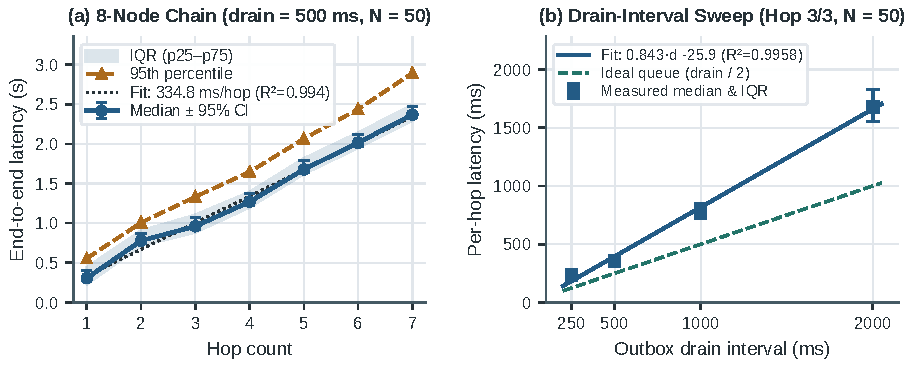
\includegraphics[width=.72\textwidth]{figures-v2/fig4-hop-and-drain-scaling.pdf}
  \caption{Hop and drain-interval scaling, 50 posts per configuration. Left: eight-node linear chain at a 500\,ms drain interval. Right: four-node drain sweep dividing hop-three median latency by three against ideal $\mathit{drain}/2$ queueing.}
  \label{fig:chain}
\end{figure*}

\begin{figure*}[!t]
  \centering
  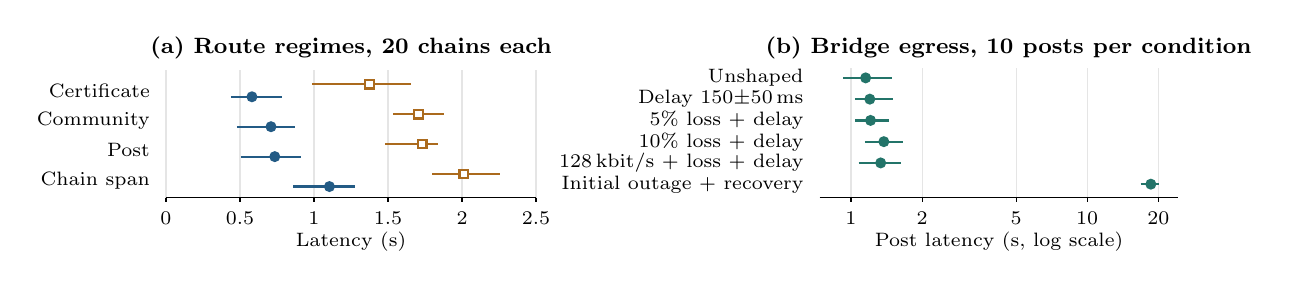
\begin{tikzpicture}[font=\scriptsize]
    % Panel (a): Route regimes
    \begin{scope}[xshift=0cm]
      \node[font=\footnotesize\bfseries] at (2.85,2.10) {(a) Route regimes, 20 chains each};
      \draw[gray!20] (0.5,0.20) -- (0.5,1.82);
      \draw[gray!20] (1.44,0.20) -- (1.44,1.82);
      \draw[gray!20] (2.38,0.20) -- (2.38,1.82);
      \draw[gray!20] (3.32,0.20) -- (3.32,1.82);
      \draw[gray!20] (4.26,0.20) -- (4.26,1.82);
      \draw[gray!20] (5.20,0.20) -- (5.20,1.82);
      \draw (0.5,0.20) -- (5.20,0.20);
      \foreach \x/\lbl in {0.5/0, 1.44/0.5, 2.38/1, 3.32/1.5, 4.26/2, 5.20/2.5} {
        \draw (\x,0.20) -- (\x,0.14) node[below] {\lbl};
      }
      \node[below=9pt] at (2.85,0.20) {Latency (s)};
      % y positions: Cert=1.56, Comm=1.18, Post=0.80, Span=0.42 (x = 0.5 + 1.88 * t)
      \node[left] at (0.42,1.56) {Certificate};
      \node[left] at (0.42,1.18) {Community};
      \node[left] at (0.42,0.80) {Post};
      \node[left] at (0.42,0.42) {Chain span};
      % Intact (blue circle, -0.08) & Bridged (amber square, +0.08)
      \draw[jbamber,thick] (2.353,1.64) -- (3.616,1.64);
      \fill[white] (3.084-0.055,1.64-0.055) rectangle (3.084+0.055,1.64+0.055);
      \draw[jbamber,thick] (3.084-0.055,1.64-0.055) rectangle (3.084+0.055,1.64+0.055);
      \draw[jbblue,thick] (1.326,1.48) -- (1.969,1.48);
      \fill[jbblue] (1.592,1.48) circle (2.0pt);

      \draw[jbamber,thick] (3.384,1.26) -- (4.033,1.26);
      \fill[white] (3.708-0.055,1.26-0.055) rectangle (3.708+0.055,1.26+0.055);
      \draw[jbamber,thick] (3.708-0.055,1.26-0.055) rectangle (3.708+0.055,1.26+0.055);
      \draw[jbblue,thick] (1.401,1.10) -- (2.143,1.10);
      \fill[jbblue] (1.834,1.10) circle (2.0pt);

      \draw[jbamber,thick] (3.285,0.88) -- (3.961,0.88);
      \fill[white] (3.755-0.055,0.88-0.055) rectangle (3.755+0.055,0.88+0.055);
      \draw[jbamber,thick] (3.755-0.055,0.88-0.055) rectangle (3.755+0.055,0.88+0.055);
      \draw[jbblue,thick] (1.453,0.72) -- (2.216,0.72);
      \fill[jbblue] (1.882,0.72) circle (2.0pt);

      \draw[jbamber,thick] (3.883,0.50) -- (4.744,0.50);
      \fill[white] (4.284-0.055,0.50-0.055) rectangle (4.284+0.055,0.50+0.055);
      \draw[jbamber,thick] (4.284-0.055,0.50-0.055) rectangle (4.284+0.055,0.50+0.055);
      \draw[jbblue,thick] (2.116,0.34) -- (2.898,0.34);
      \fill[jbblue] (2.576,0.34) circle (2.0pt);
    \end{scope}

    % Panel (b): Bridge egress netem (x = 9.2 + 3.0 * log10(t))
    \begin{scope}[xshift=0cm]
      \node[font=\footnotesize\bfseries] at (11.2,2.10) {(b) Bridge egress, 10 posts per condition};
      \foreach \xt in {9.200, 10.103, 11.297, 12.200, 13.103} {
        \draw[gray!20] (\xt,0.20) -- (\xt,1.85);
      }
      \draw (8.80,0.20) -- (13.35,0.20);
      \foreach \xt/\lbl in {9.200/1, 10.103/2, 11.297/5, 12.200/10, 13.103/20} {
        \draw (\xt,0.20) -- (\xt,0.14) node[below] {\lbl};
      }
      \node[below=9pt] at (11.08,0.20) {Post latency (s, log scale)};
      \node[left] at (8.72,1.72) {Unshaped};
      \node[left] at (8.72,1.45) {Delay 150$\pm$50\,ms};
      \node[left] at (8.72,1.18) {5\% loss + delay};
      \node[left] at (8.72,0.91) {10\% loss + delay};
      \node[left] at (8.72,0.64) {128\,kbit/s + loss + delay};
      \node[left] at (8.72,0.37) {Initial outage + recovery};

      \draw[jbteal,thick] (9.104,1.72) -- (9.721,1.72);
      \fill[jbteal] (9.386,1.72) circle (2.0pt);
      \draw[jbteal,thick] (9.250,1.45) -- (9.734,1.45);
      \fill[jbteal] (9.439,1.45) circle (2.0pt);
      \draw[jbteal,thick] (9.252,1.18) -- (9.682,1.18);
      \fill[jbteal] (9.448,1.18) circle (2.0pt);
      \draw[jbteal,thick] (9.376,0.91) -- (9.864,0.91);
      \fill[jbteal] (9.617,0.91) circle (2.0pt);
      \draw[jbteal,thick] (9.298,0.64) -- (9.831,0.64);
      \fill[jbteal] (9.577,0.64) circle (2.0pt);
      \draw[jbteal,thick] (12.879,0.37) -- (13.108,0.37);
      \fill[jbteal] (13.008,0.37) circle (2.0pt);
    \end{scope}
  \end{tikzpicture}
  \caption{Median latency and 95\% bootstrap intervals. In~(a), filled circles mark the intact exchange and open squares the bridged route. In~(b), all 10 posts arrived under each condition; delay is configured egress delay, and the interruption batch was queued prior to the first recovery.}
  \label{fig:netem}
\end{figure*}

\begin{table*}[!t]
  \caption{Admission Under Load. Memory Snapshots Were Sampled After Each Valid-Write Batch.}
  \label{tab:load}
  \centering
  {\footnotesize
  \begin{tabular}[t]{@{}lrr@{}}
    \multicolumn{3}{@{}l}{\textbf{(a) HTTP admission at concurrency 16}} \\
    \toprule
    Request batch & Requests/s & Median (ms) \\
    \midrule
    Invalid input, default HTTP limit & 1,347 & 6.01 \\
    Invalid input, raised HTTP limit & 293 & 55.31 \\
    Malformed protobuf & 2,383 & 5.87 \\
    Exact duplicate & 159 & 92.45 \\
    Reused nonce & 134 & 116.06 \\
    \bottomrule
  \end{tabular}\hspace{1.4cm}%
  \begin{tabular}[t]{@{}rrrrr@{}}
    \multicolumn{5}{@{}l}{\textbf{(b) Valid writes, 200 posts total per setting}} \\
    \toprule
    & & \multicolumn{2}{c}{Latency (ms)} & Node memory \\
    Concurrency & Requests/s & Median & p95 & (MiB) \\
    \midrule
    1 & 29 & 32.06 & 49.41 & 108 \\
    4 & 27 & 104.33 & 352.60 & 133 \\
    16 & 9 & 1,300.69 & 4,132.36 & 175 \\
    32 & 6 & 4,192.33 & 12,586.59 & 181 \\
    \bottomrule
  \end{tabular}}
\end{table*}

\section{Methodology}
\label{sec:method}

Controlled experiments ran on one physical x86\_64 Linux host (Intel Core i5-8265U, 8 logical CPUs, 19.38\,GiB RAM, Linux 7.2.14, Docker 29.9.2) running \texttt{node:20-alpine}, MongoDB~7, and Redis~7 containers. The route-cut, impairment, stress, and scaling experiments used a configuration without steady-state pull. Differential validation, the automated route-cut validation test, and the ActivityPub and blocked-inbound runs used a configuration with steady-state pull, bounded gRPC cancellation, and author-signature verification by the ALS.

\textbf{Route-cut topology and validation.} The testbed consisted of four application nodes (A1 and A2 on island~A, B1 on island~B, and the dual-homed bridge), two MongoDB instances isolated by island, and two Redis caches. It used three internal Docker networks for island~A, island~B, and the shared exchange. The automated route-cut validation test checked the bridge's TCP sockets for both configured uplink IP addresses, disconnected the exchange links, and verified DNS isolation between A1 and B1. Before submitting the test post, we confirmed that B1 did not already have it. The test polled for post arrival, relay counters, reserved forwarding capacity, and uplink failover and recovery.

\textbf{Measurements and impairment experiments for the route-cut topology.} We sent 20 dependency chains (author certificate, community record, and post) with the exchange intact. We then severed the direct exchange link once and sent 20 more chains through the bridge on the same running stack. Each chain used a fresh identity and community. To measure propagation delay independently of polling, we subtracted the source \texttt{received\_at\_ms} timestamp from the destination timestamp using the shared host clock. Chain duration ran from insertion of the source certificate to insertion of the destination post. We report medians, interquartile ranges (IQRs), sample standard deviations (SDs), and 95\% within-run percentile bootstrap confidence intervals for the medians (10,000 resamples). In the bridged topology, \texttt{tc prio} and \texttt{u32} filters applied impairments only to bridge federation traffic on TCP port~8444. Database traffic stayed unshaped. We tested 10 posts per condition across one unshaped control and five impairment conditions.

\textbf{Scaling and admission stress.} Linear chains isolated hop count with 50 posts per configuration: an eight-node chain at a 500\,ms drain interval and a four-node drain sweep across 250, 500, 1,000, and 2,000\,ms (with start and end 500\,ms controls). Each node used a distinct logical database inside one shared MongoDB process, so measurements include shared-process contention; a separate 200-envelope run used a 1,000\,ms drain interval. Stress runs exercised HTTP admission, malformed protobufs, exact duplicates, non-idempotent nonce reuse, 5-peer gRPC frames/quotas, and single-node valid writes (32 certified identities, 200 posts per concurrency level), recording status codes, latencies, collection deltas, MongoDB profiler writes, and Docker CPU/memory snapshots.

\textbf{ActivityPub comparison.} Two Jagoo Bahee nodes were paired with two minimal Node.js HTTP-inbox peers implementing gzip, Ed25519 HTTP Signatures, and push retries, with isolated database and WAN interfaces. WAN shaping added 75\,ms delay ($\pm$15\,ms) per direction, 5\% loss, and a 128\,kbit/s rate cap. We recorded sender WAN interface transmit bytes (including framing and any background packets). For Jagoo Bahee, we measured delivery time from insertion into the source database to insertion into the destination database. For the minimal inbox, timing began before the sender compressed and signed the payload and ended at verified in-memory receipt. Separately, we created 40 synthetic posts with public visibility on a local Mastodon 4.7.6 instance running in Docker. We retrieved their \texttt{Create} activities from the outbox, restored \texttt{@context} from each corresponding standalone \texttt{Note}, and measured the compact JSON and gzipped sizes. We subtracted authored UTF-8 text bytes from the raw size to obtain non-text bytes.

\section{Results}
\label{sec:results}

\subsection{Decoding, route cuts, and impairment}

The TypeScript, Rust, and Python implementations produced identical bytes for 16 canonical reference vectors and showed no disagreements across 20,000 seeded differential cases. Across 10,000 generated wire-format inputs (numeric boundaries, Unicode normalization cases, and empty anti-abuse variants), all three implementations matched on canonical bytes, content identifiers, and round-trip decoding. Across 16 mutation classes (10,000 cases), all three decoders jointly rejected 9,455 inputs and identically decoded the 545 mutated inputs they accepted with zero disagreements. These tests evaluate wire-format agreement rather than signature verification, application admission, or full protocol security.

The automated route-cut validation test passed all 22 checks in 39.91\,s. In the measurements before and after the route cut (Figs.~\ref{fig:topology} and \ref{fig:netem}a), island~B received 20/20 certificates, communities, and posts in both regimes. Median post latency rose from 735\,ms (IQR 436\,ms, 95\% CI 507--913\,ms, SD 260\,ms) with the exchange intact to 1,732\,ms (IQR 446\,ms, CI 1,482--1,841\,ms, SD 298\,ms) via the bridge. Certificate and community medians were 581 and 710\,ms intact (CIs 440--782 and 479--874\,ms) versus 1,375 and 1,707\,ms bridged (CIs 986--1,658 and 1,534--1,879\,ms); median chain span rose from 1,105 to 2,013\,ms (bridged CI 1,800--2,258\,ms).

\begin{table*}[!t]
  \caption{Object Sizes, Delivery Latency, and Sender-Interface Traffic. Panel (a) gives Mastodon medians and Jagoo Bahee examples.}
  \label{tab:ap}
  {\footnotesize\noindent
  \begin{tabular*}{0.48\textwidth}[t]{@{\extracolsep{\fill}}lrrr@{}}
    \multicolumn{4}{@{}l}{\textbf{(a) Object representations (bytes)}} \\
    \toprule
    Source & Full raw & Non-text raw & Full gzip \\
    \midrule
    Local Mastodon ($n=40$) & 3,385 & 3,148 & 811.5 \\
    Jagoo Bahee check-in & 155 & 155 & --- \\
    Jagoo Bahee broadcast & 243 & 177 & --- \\
    Jagoo Bahee post & 220 & 206 & --- \\
    \bottomrule
  \end{tabular*}\hfill%
  \begin{tabular*}{0.48\textwidth}[t]{@{\extracolsep{\fill}}lrr@{}}
    \multicolumn{3}{@{}l}{\textbf{(b) Delivery under asymmetric reachability}} \\
    \toprule
    Delivery method & Delivered & Median (ms) \\
    \midrule
    \multicolumn{3}{@{}l}{\emph{Inbound federation traffic blocked, shaping disabled}} \\
    Jagoo Bahee periodic pull & 10/10 & 1,045.5 \\
    Minimal inbox push & 0/10 & --- \\
    \multicolumn{3}{@{}l}{\emph{Jagoo Bahee with listener disabled}} \\
    Backfill from startup & 10/10 & 4,957 \\
    Outbound push & 10/10 & 340.5 \\
    \bottomrule
  \end{tabular*}

  \vspace{6pt}\noindent
  \begin{tabular*}{\textwidth}[t]{@{\extracolsep{\fill}}llrrr@{}}
    \multicolumn{5}{@{}l}{\textbf{(c) Delivery on the shaped link} (128\,kbit/s, 5\% packet loss, 75\,ms added delay per direction)} \\
    \toprule
    System & Timed interval & Delivered & Median (ms) & Sender interface (B/post) \\
    \midrule
    Jagoo Bahee & Origin insertion to destination insertion & 20/20 & 520.5 & 1,846.4 \\
    Minimal inbox & Sender delivery routine to in-memory receipt & 20/20 & 154.5 & 1,278.3 \\
    \bottomrule
  \end{tabular*}}
\end{table*}

All 10 posts reached the destination in each of the six network-emulation scenarios (Fig.~\ref{fig:netem}b). Median post latency was 1.154\,s in the unshaped control and 1.202\,s with 150$\pm$50\,ms of added egress delay. The median was 1.210\,s with 5\% packet loss and 50$\pm$15\,ms delay, 1.377\,s with 10\% loss and 75$\pm$25\,ms delay, and 1.335\,s with a 128\,kbit/s cap, 50$\pm$10\,ms delay, and 2\% loss. In the intermittent-loss test, we queued all 10 posts while the bridge's island-B uplink dropped all packets. After queuing, we held full loss for 8\,s before the first 8\,s recovery window, then repeated the loss and recovery cycle twice. Median delivery latency was 18.595\,s (95\% CI 16.841--20.071\,s).

\subsection{Scaling, stress, and resource use}

The eight-node chain delivered 50/50 posts at every hop with a 500\,ms drain interval (Fig.~\ref{fig:chain}). At hop seven, median latency was 2.368\,s (95\% CI 2.332--2.469\,s, IQR 0.191\,s, p95 2.893\,s). Median latency increased by a fitted 335\,ms per hop ($R^2 = 0.994$). In the four-node sweep, all 50 posts arrived at each setting. Hop-three medians were 0.707, 1.067, 2.365, and 5.035\,s at drain intervals of 250, 500, 1,000, and 2,000\,ms, respectively. Dividing each hop-three median by three gave an estimated per-hop latency that increased by 0.843\,ms per millisecond of drain interval ($R^2 = 0.996$). The hop-three median for the repeated 500\,ms control rose by 10.9\% from the start to the end of the sweep. In a separate 200-envelope run with a 1,000\,ms drain interval, hop-seven latency had a median of 4.125\,s and a p99 of 6.115\,s.

At HTTP concurrency~16 (Table~\ref{tab:load}a), the default limiter rate-limited 2,709 of 3,000 invalid requests. The batch ran at 1,347\,req/s with a median response time of 6.01\,ms. With the limit raised, the server rejected 2,593 of 3,000 requests for bad signatures, and the batch ran at 293\,req/s with a median of 55.31\,ms. Malformed protobuf inputs produced 3,000 HTTP~400 responses and zero HTTP~500 errors (2,383\,req/s). The server returned existing receipts for all 1,000 exact duplicates (159\,req/s) and HTTP~409 replay rejections for all 1,000 nonce-reuse requests in the non-idempotent vote domain (134\,req/s). The MongoDB profiler recorded zero writes in the five HTTP batches. In a separate gRPC test across five peers, the receiver rejected all 500 frames, including 407 with bad-signature errors. In the over-quota rounds, the receiver blocked two peers, made 15 writes to peer state, and accepted no envelopes.

In the single-node tests with valid writes (Table~\ref{tab:load}b), all 200 posts at each concurrency setting reached the local projection. Raising concurrency from 1 to 32 reduced throughput from 29 to 6\,requests/s while increasing median latency from 32.06 to 4,192.33\,ms, p95 from 49.41 to 12,586.59\,ms, and p99 from 60\,ms to 15.940\,s. These figures characterize local single-node admission scalability under shared storage rather than concurrent end-to-end federation capacity; we did not profile per-stage CPU/lock time to isolate a single bottleneck. Node container memory snapshots grew from 87\,MiB idle to 108--181\,MiB after valid-write batches (MongoDB 150--345\,MiB, Redis $<9.5$\,MiB). Eight-node chain containers used 77--111\,MiB each (max sampled CPU 21.18\%; shared MongoDB 184\,MiB, Redis 9\,MiB), and active route-cut nodes used 105--151\,MiB (0.59--30.72\% CPU).

\subsection{ActivityPub and blocked-inbound delivery}

On the constrained lossy link, Jagoo Bahee and the minimal ActivityPub inbox each delivered 20/20 posts (Table~\ref{tab:ap}). Jagoo Bahee recorded a median delivery time of 520.5\,ms (95\% CI 394--586\,ms), 1,846.4 bytes per post at the sender's network interface, and container memory snapshots of 88--92\,MiB. The minimal inbox recorded a median of 154.5\,ms (95\% CI 145--161\,ms), 1,278.3 bytes per post at the sender's interface, and memory snapshots of 9--14\,MiB. These measurements apply to the tested implementations. The timers cover different operations, and the minimal inbox receives posts in memory and omits Mastodon's web and worker stack.

With shaping disabled, inbound federation ports blocked at the receivers, and outbound connections available, the minimal push-only inbox delivered 0/10 posts within its retry budget. Jagoo Bahee's periodic pull recovered 10/10 posts with a median delivery time of 1.046\,s (95\% CI 0.469--1.509\,s). In a separate run, an outbound-only node with its gRPC listener disabled backfilled 10/10 existing posts with a median of 4.957\,s from startup and pushed 10/10 new posts with a median of 0.341\,s.

The 40 synthetic Mastodon posts had median representation sizes of 3,385\,B raw and 811.5\,B gzipped, with 3,148\,B of non-text data in the raw representation. The Jagoo Bahee check-in, broadcast, and forum-post examples contained 155, 177, and 206\,B of non-text data, respectively. These objects carry different fields. Sender-interface traffic also includes framing and synchronization traffic (Table~\ref{tab:ap}).

\section{Discussion and Limitations}
\label{sec:limits}

\textbf{Implications.} When domestic IP routes remain available, the protocol can verify and deliver messages between islands. This adds work for validation and storage and may require extra relay hops. If inbound connections are blocked, a node can still pull queued messages from a peer whose address it knows and can reach. Network traffic includes signed payloads, framing, receipts, and synchronization messages.

\textbf{Testbed and measurement limits.} All experiments share one x86\_64 host kernel, clock, CPU, and storage stack. Because intact route trials ran before the bridge trials on the same stack, route effects cannot be separated from host-load drift. Replicating the topology across independent machines requires measuring inter-host clock skew, physical routing, variable access links, and wide-area latency. Peak resident memory, disk growth, sustained resource-exhaustion limits, and single-board computer performance remain unmeasured.

\textbf{Deployment and security limits.} When providers block communication between subscribers, affected nodes can operate only locally. Cross-island federation stops when every IP path between the islands is lost. Backfill rejects envelopes created more than seven days before receipt, according to the receiver's clock. Long partitions can therefore leave gaps in the recovered history. The relay binds each outbound connection to the source IP address of its chosen uplink. Network operators can observe endpoint addresses and communication timing, and protocol allowlists can block gRPC. The system offers no anonymity guarantee. Forum operators choose whether to acknowledge admission or relay an object. An originating server with lenient admission rules can admit many valid objects under its own policy, leaving receiving peers to enforce their ingress quotas.

\section{Conclusion}

We demonstrated that exact-byte admission, verifiable receipts, caller-initiated synchronization, and quota-bounded validating relays can support federated communication over surviving IP paths. In a single-host Docker testbed, dependent signed objects crossed between islands through a dual-homed bridge after we withdrew the direct path through the shared exchange. All posts arrived in each controlled network-emulation scenario, and periodic pull recovered all queued posts in the test with inbound federation ports blocked. In separate tests, single-node admission throughput fell as write concurrency rose, and the prototype used more sender-side network bytes per post than a minimal ActivityPub push inbox on a constrained lossy link.

\bibliographystyle{IEEEtran}
\bibliography{iccit2026-paper-pre-references}

\end{document}
